\subsection{Complete-work correction on molecular rotors}\label{sec:rotor-work}
To test the work correction directly, we select three methyl rotors from training
molecules in fixed data order, using geometry alone.
Each rotor turns the three hydrogens of a methyl group around its bond axis while
holding the other internal coordinates fixed. The rotation angle $\phi$ therefore
specifies a one-dimensional family of three-dimensional molecular structures.
A periodic interpolant of 512 GFN2 energies supplies their potential $U(\phi)$;
$U(0)$ is the reference energy at angle zero. The target is
$\rho(\phi)\propto q_0(\phi)\exp[-(U(\phi)-U(0))/kT]$, where $q_0$ is a normalized
von Mises reference of concentration one: a smooth circular distribution favoring
angles near zero. The product retains this reference restraint and gives greater
weight to lower-energy angles. Here $kT=k_B T_{\rm phys}$ at 300 K.

Starting from $\phi\sim q_0$, use escorts $\psi_a(\phi)=\phi+a\sin\phi$ for
$a\in\{-0.5,0,0.5\}$. Their positive Jacobian is $J_a=1+a\cos\phi$.
The map $\psi_a$ changes the sampled angle; $a$ sets its strength, and $J_a$
measures how it locally expands or compresses angular intervals. The complete
generalized work includes both reference densities and $-kT\log J_a$
(Appendix~\ref{app:rotor-work}). We compare complete work, energy-only weights,
weights omitting the Jacobian, and unweighted endpoints, with shared draws and
128 repetitions at each of 8, 32, 128, 512 and 2,048 samples.

\begin{figure}[t]
\centering
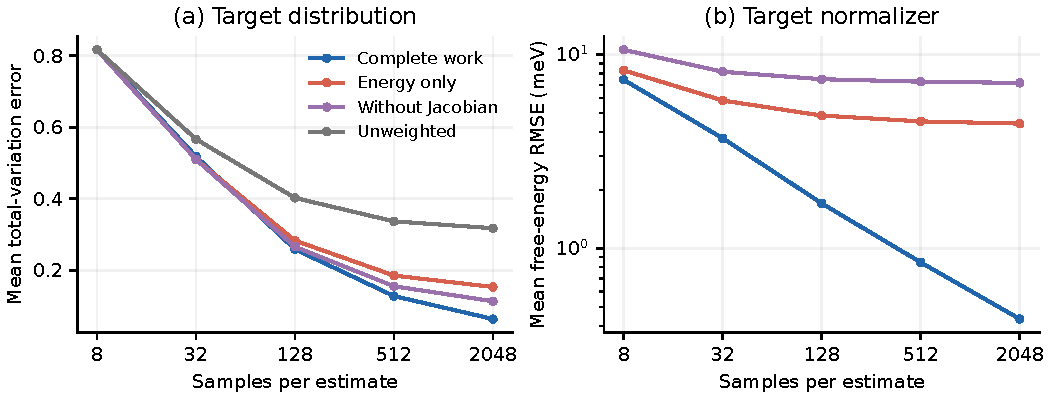
\includegraphics[width=\linewidth]{../research/figures/rotor_work_v1/rotor_work.pdf}
\caption{Complete work corrects the nonequilibrium sampling bias on the specified
torsional targets. Curves average all three molecules and both nonidentity
escorts; each case has 128 repetitions. Energy-only and incomplete-work controls
retain bias as sampling increases. Unweighted endpoints have no free-energy
estimator. Each target is a constrained molecular rotor at 300 K.}\label{fig:rotor-work}
\end{figure}

Total variation measures disagreement between the estimated and target angular
probabilities, with zero indicating agreement. Free-energy RMSE measures error in
the logarithm of the target normalizer, expressed in energy units.

At 2,048 samples, complete work has lower mean total-variation error than both
incomplete-weight controls in all six nonidentity cases. Across these cases,
mean errors are 0.0636 for complete work, 0.1532 for energy-only weights and
0.1134 without the Jacobian, a 58.5\% reduction relative to energy-only weighting.
Complete-work free-energy RMSE ranges from 0.158 to 0.734 meV. Independent
density-ratio quadrature also recovers the specified target normalizer in all
nine molecule/escort cases. The identity-escort control makes the three weighted
methods coincide. Together, the distribution and normalizer results show the
role of complete work accounting on these molecular energy curves.
